\section{mCRL System Behaviour Modelling}
This section elaborates on the model that was modelled for the boat lift in mCRL2. The complete code can be found within Appendix A.
\subsection{The code}
The code has been divided into four controllers: one master controller and three sub controllers. Namely gate, valve and signal controller discussed in the previous section. The communication between each controller to the master and vice versa are clarified in Figure \ref{fig:subcontrollers}.
Series of data types have been defined and used in the model which can be seen in Table \ref{tab:sort}.

\begin{table}[htbp]
	\centering
	\begin{tabular}{lp{10.5cm}l}
		\toprule
		\textbf{Sort} &  \textbf{Description} \\
		\hline
		State&  Defines states of the master controller \\
		M2G &  Defines communication elements from the master to gate controller\\
		G2M & Defines communication elements from the gate to master controller \\
		M2S &  Defines communication elements from the master to signal controller\\
		S2M &  Defines communication elements from the signal to master controller\\
		M2V &  Defines communication elements from the master to valve controller\\
		V2M &  Defines communication elements from the valve to master controller\\
		SLID &  Defines signal light IDs\\
		GateID &  Defines gate IDs\\
		ValveID &  Defines valve IDs\\
		PositionID   & Defines position IDs\\
		\bottomrule
	\end{tabular}%
		\caption{Sorts/Data types of the model}
	\label{tab:sors}%
\end{table}%
 There are multiple states were each of them represents an action, or a series of a few very related actions, and then it switches to the next state. But befure going to the next state the mastercontroller checks the correctness of the current state and then goes on the the next one or it creates a loop to the same state to keep checking. When a ship leaves the lift, the loop of the states can go back to idle or create a more complex loop depending on boats waiting to use the lift. This state forwarding mechanism allows the master controller to receive reliable information about the status of the systems from the other sub-controllers at any time. The initial state of the boat lift is by definition idle state were the lift can expect a boat from either side.\\
During the writing of the mCRL2 code, the graph and the view tools were mostly used for analyzing as well as branching bisimulation. When looking at the view in Figure \ref{fig:view}, the system can be analyzed and explained efficiently. The model is mainly composed of two main branches that start from the idle state, they describe a boat going up the lift and a boat going down the lift. The system goes into one state at a time going down the branch. This method is effective to fulfill all requirement which will be checked and verified in the next Chapter. 

\begin{figure}[!h]
	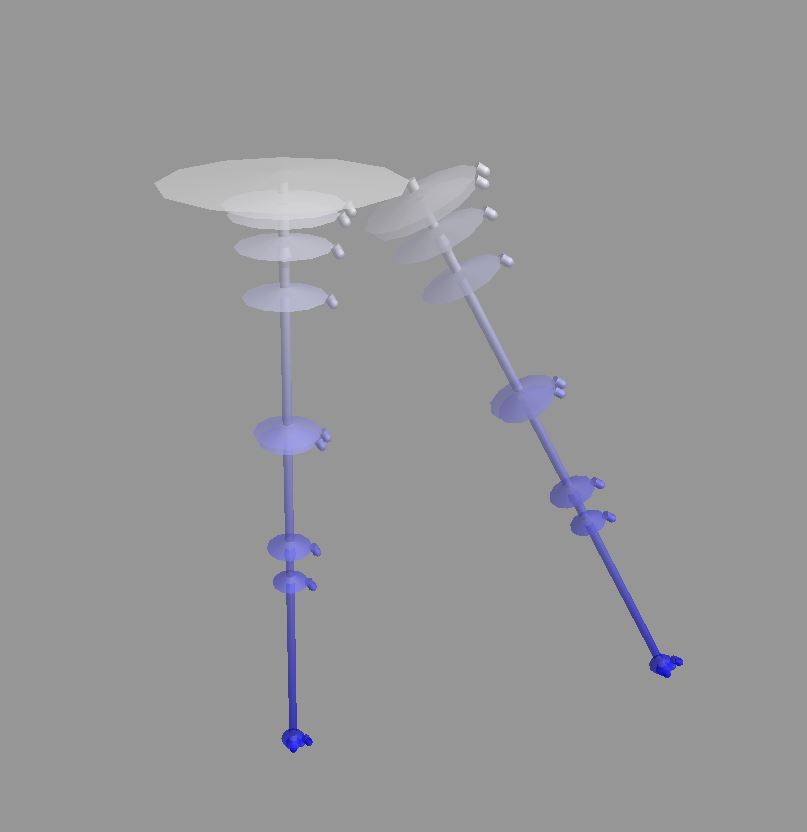
\includegraphics[width=\linewidth]{view}
	\caption{The view tool in mCRL2 shows efficiently how the model is structured}
	\label{fig:view}
\end{figure}

%Moreover, in the tools is it possible to look that many states has some loops needed for two reasons: for the sub-controllers to check all the boat lift state and for the master for check for response from valve, gate and signal sub controllers.

